\documentclass[11pt,a4paper, 
swedish, english %% Make sure to put the main language last!
]{article}
\pdfoutput=1

%% Andréas's custom package 
%% (Will work for most purposes, but is mainly focused on physics.)
\usepackage{../custom_as}
\usepackage{mathrsfs}
\usepackage{eufrak}
\usepackage{cancel}
%% Figures can now be put in a folder: 
\graphicspath{ {figures/} %{some_folder_name/}
}
\usepackage{multicol}

%% If you want to change the margins for just the captions
\usepackage[size=small]{caption}

%% To add todo-notes in the pdf
\usepackage[%disable  %%this will hide all notes
]{todonotes} 

%% Change the margin in the documents
\usepackage[
%            top    = 3cm,              %% top margin
%            bottom = 3cm,              %% bottom margin
%            left   = 3cm, right  = 3cm %% left and right margins
]{geometry}

\newcommand{\enull}{\ensuremath{\varepsilon_{0}}}
\newcommand{\lD}{\ensuremath{\lambda_{\text{D}}}}
\newcommand{\wc}{\ensuremath{\omega_{\text{c}}}}
\newcommand{\rhom}{\ensuremath{{\rho_{\text{m}}}}}


%% If you want to chage the formating of the section headers
\renewcommand{\thesubsection}{\arabic{section}.\Alph{subsection}}



%%%%%%%%%%%%%%%%%%%%%%%%%%%%%%%%%%%%%%%%%%%%%%%%%%%%%%%%%%%%%%%%%%%%%%
\begin{document}%% v v v v v v v v v v v v v v v v v v v v v v v v v v
%%%%%%%%%%%%%%%%%%%%%%%%%%%%%%%%%%%%%%%%%%%%%%%%%%%%%%%%%%%%%%%%%%%%%%


%%%%%%%%%%%%%%%%%%%% vvv Internal title page vvv %%%%%%%%%%%%%%%%%%%%%
\title{Assignment 4 \\
{\Large Plasma Physics -- RRY085}}
\author{Andréas Sundström}
\date\today%{2017-10-01}

\maketitle

%%%%%%%%%%%%%%%%%%%% ^^^ Internal title page ^^^ %%%%%%%%%%%%%%%%%%%%%
%% If you want a list of all todos
%\todolist

\section{Collisional diffusion in weakly ionized gas}
Assume that the electron-neutral interaction rate is
\begin{equation}
\nu_{\text{en}}=v_\ee N \sigma_\text{en},
\end{equation}
and the electron-ion interaction rate is
\begin{equation}
\nu_\text{ei}=\frac{\pi n e^4}{(4\pi\varepsilon_0 m_\ee)^2v_\ee^3},
\end{equation}
where $N$ is the neutral particle density and $n=n_\ee=n_\text{i}$ is
the electron/ion density. Then
\begin{equation}
\frac{\nu_\text{ei}}{\nu_{\text{en}}}
=\frac{n}{N}\frac{e^4}
{16\pi\varepsilon_0^2\sigma_\text{en}m_\ee^2 v_\ee^4}.
\end{equation}
If we take $\sigma_\text{en}=\unit[10^{-19}]{m^2}$ and an electron
energy of 1\,eV, then for the two different frequencies to be equal,
we would require 
\begin{equation}
\frac{n}{N}=
\frac{64\pi\varepsilon_0^2
\sigma_\text{en}\,\epsilon^2}{e^4}
\approx 0.06 = 6\,\%,
\end{equation}
where $\epsilon =m_\ee v_\ee^2/2$ is the energy of an electron.

Given air normal atmospheric pressure at room temperature with
$N=\unit[10^{26}]{m^{-3}}$ and weakly ionized plasma, and with the
same electron energy and $\sigma_\text{en}$. Then the diffusion
constant is roughly 
\begin{equation}
D=\frac{v_\ee^2}{\nu_\text{en}}
=\frac{v_\ee}{N\sigma_\text{en}}
=\frac{1}{N\sigma_\text{en}}\sqrt{\frac{2\epsilon}{m_\ee}}
\approx \unit[0.06]{m^2/s}.
\end{equation}
Since the plasma would be weakly ionized the electron-neutral
collision rate dominates. 



\section{Different heat conductivity models}
In this problem we're considering a 1D plasma system, and we will
investigate how different types of heat conductivity, $\chi$, will
affect the temperatures of the plasma. The temperature is given by the
ODE
\begin{equation}
\dv{r}\qty[\chi\dv{T}{r}]=-S(r)\qc
\eval{\dv{T}{r}}_{r=0}=0\qc
T(r=R)=T_0,
\end{equation}
where $S(r)=S_0(r-r_0)$ with $0<r_0<R$. With this information, we can
integrate both sides once
\begin{equation}\label{eq2:ODE}
\chi\dv{T}{r}=-S_0\Theta(r-r_0),
\end{equation}
where $\Theta$ is the Heaviside step function. There should also be a
constant of integration here, but with the initial condition
$\eval{\dv*{T}{r}}_{r=0}=0$, we see that said constant has to be~0
(unless $\chi$ diverges at $r\to0$).

Seeing that we will be dealing with the Heaviside step function, we
might as well state the following identity for integration with the
step function. Given some (smooth) function $f(x')$ and the constants
$x_1<x_0$, then 
\begin{equation}
\begin{aligned}
\int_{x_1}^{x}\dv{f}{x'}\Theta(x'-x_0)\id{x'}=&
\Theta(x-x_0)\int_{x_0}^{x}\dv{f}{x'}\id{x'}
=\Big(f(x)-f(x_0)\Big)\Theta(x-x_0).
\end{aligned}
\end{equation}
Obviously, any primitive function to $(\dv*{f}{x'})\Theta(x'-x_0)$
will be given by the RHS plus some arbitrary constant, thus
\begin{equation}\label{eq2:heaviside-int}
\int\dv{f}{x}\Theta(x-x_0)\id{x}
=C+\Big(f(x)-f(x_0)\Big)\Theta(x-x_0).
\end{equation}



\subsection{Classical transport}
If the heat conductivity follows classical heat transport, then
\begin{equation}
\chi(T)=\alpha_1T^{-1/2}
\end{equation}
and \eqref{eq2:ODE} is separable and we get
\begin{equation}
\int\alpha_1T^{-1/2}\id{T}=-\int S_0\Theta(r-r_0)\id{r},
\end{equation}
which, by \eqref{eq2:heaviside-int}, becomes
\begin{equation}
T^{1/2}(r)=\mathcal{T}^{1/2}
-\frac{S_0}{2\alpha_1}(r-r_0)\Theta(r-r_0).
\end{equation}
The constant of integration, $\mathcal{T}^{1/2}$, can easily be
determined by the boundary condition $T(r=R)=T_0$ which yields
\begin{equation}\label{eq2a:const}
T_0^{1/2}=\mathcal{T}^{1/2}-\frac{S_0}{2\alpha_1}(R-r_0)
\quad\Longleftrightarrow\quad
\mathcal{T}^{1/2}=T_0^{1/2}+\frac{S_0}{2\alpha_1}(R-r_0).
\end{equation}
This means that the temperature is
\begin{equation}
T(r)=\qty{T_0^{1/2}+\frac{S_0}{2\alpha_1}
\Big[(R-r_0)-(r-r_0)\Theta(r-r_0)\Big]}^2
\end{equation}
With words, the temperature stays constant $T=\mathcal{T}$, given by
\eqref{eq2a:const}, up until $r=r_0$ when the temperature drops 
``quadratically'' (along a parabola whose vertex is just to the right
of $r=R$) down to $T=T_0$ at $r=R$. 

\subsection{Neoclassical transport}
With neoclassical transportation, the heat conductivity is
\begin{equation}
\chi(r, T)=
\begin{cases}
\alpha_2 r_1^{-3/2}T^{-1/2}\qc&0\le r<r_1\\
\alpha_2 r^{-3/2}T^{-1/2}\qc& r_1\le r\le1,
\end{cases}
\end{equation}
where $0<r_1<r_0$. 

It is obvious that the tempereature, just as before, will be constant
$T(r)=\mathscr{T}$ for $0\le r<r_0$ since $\dv*{T}{r}=0$ in that region. We
can therefore focus on the region $r_0<r<R$. There \eqref{eq2:ODE} can
be rewritten as 
\begin{equation}
\alpha_2T^{-1/2}\dv{T}{r}=-S_0\,r^{3/2}\Theta(r-r_0)=-S_0\,r^{3/2}
\end{equation}
which separates into
\begin{equation}
\alpha_2\int T^{-1/2}\id{T}=-S_0\int r^{3/2}\Theta(r-r_0) \id{r}.
\end{equation}
By \eqref{eq2:heaviside-int}, we therefore get
\begin{equation}
T^{1/2}(r)=\mathscr{T}^{1/2}
-\frac{S_0}{5\alpha_2}\qty(r^{5/2}-r_0^{5/2})\Theta(r-r_0).
\end{equation}
Once again, the constant $\mathscr{T}^{1/2}$ is determined by the boundary
condition $T(r=R)=T_0$, which yields
\begin{equation}
\mathscr{T}^{1/2}=T_0^{1/2}+
\frac{S_0}{5\alpha_2}\qty(R^{5/2}-r_0^{5/2}).
\end{equation}
Therefore
\begin{equation}
T(r)=\qty{T_0^{1/2}+\frac{S_0}{5\alpha_2}
\qty[\qty(R^{5/2}-r_0^{5/2})-\qty(r^{5/2}-r_0^{5/2})\Theta(r-r_0)]}^2.
\end{equation}
This is harder to describe with words, but the temperature is constant
$T=\mathscr{T}$ for $0\le r<r_0$ and then it starts droppting down to
$T(R)=T_0$. 

\subsection{Turbulent Gyro-Bohm like transport}
For turbulent Gyro-Bohm like transport, the heat conductivity is given
by
\begin{equation}
\chi(T)=\alpha_3 T^{3/2}.
\end{equation}
Therefore, \eqref{eq2:ODE} separates into
\begin{equation}
\alpha_3\int T^{3/2}\id{T}=-S_0\int \Theta(r-r_0) \id{r}.
\end{equation}
As usual, \eqref{eq2:heaviside-int} gives
\begin{equation}
T^{5/2}(r)=\mathfrak{T}^{5/2}
-\frac{5S_0}{2\alpha_3}\qty(r-r_0)\Theta(r-r_0).
\end{equation}
The boundary condition $T(r=R)=T_0$ yields
\begin{equation}
\mathfrak{T}^{5/2}=T_0^{5/2}+
\frac{5S_0}{2\alpha_3}\qty(R-r_0)
\end{equation}
wherefore
\begin{equation}
T(r)=\qty{T_0^{5/2}+\frac{5S_0}{2\alpha_3}
\Big[(R-r_0)-(r-r_0)\Theta(r-r_0)\Big]}^{2/5}.
\end{equation}
Once again, this is constant $T=\mathfrak{T}$ for $0\le r<r_0$, and
then the temperature drops down to $T_0$ at $r=R$.

\subsection*{Limiting type of transport}
\begin{figure}
\centering\vspace{-1.9cm}
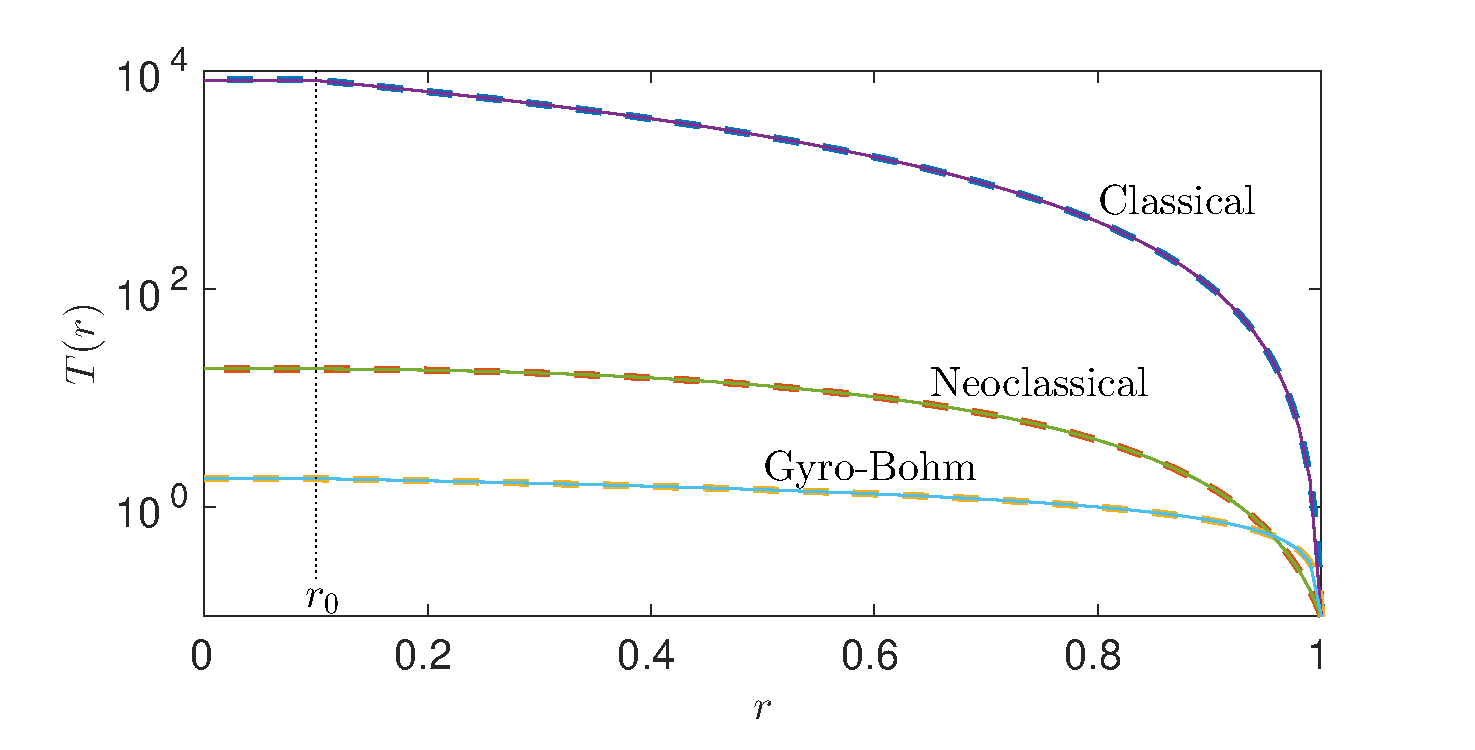
\includegraphics[width=12cm]{Q2.eps}
\caption{Temperature profiles for the three different types of heat
  transport, using the dimensionless values $S_0=10$, $R=1$,
  $r_0=0.1$, $T_0=0.1$, $\alpha_1=0.05$, $\alpha_2=0.5$ and
  $\alpha_3=5$. Also in the figure are numerical solutoins to the
  differential equations shown as thick, dashed lines. Note the log
  scale on the vertical axis.}
\label{fig:transp}
\end{figure}

Using the dimensionless values $S_0=10$, $R=1$, $r_0=0.1$, $T_0=0.1$,
$\alpha_1=0.05$, $\alpha_2=0.5$ and $\alpha_3=5$. The core temperature
for the three different scenarios can be calculated to
\begin{equation}
\mathcal{T}\approx8\,160\qc
\mathscr{T}\approx18.5\qc
\mathfrak{T}\approx1.83,
\end{equation}
for classical, neoclassical and Gyro-Bohm transoprt
respectively. We clearly see that classical transport would have
yielded the, by almost three orders of magnitude, highest core
tempereature, and that Gyro-Bohm yields the lowest core
temperature. This can also be seen in \figref{fig:transp}, where the
different temperatrue profiles have been plotted. 


\section{MHD stability}
Starting from the ideal MHD equations
\vspace{-22pt}
\begin{multicols}{2}
\begin{subequations}
\begin{align}
\label{eq:MHD-a}
&\rhom\dv{\vb*U}{t}=\vb*J\cross\vb*B-\grad P
\\ \label{eq:MHD-b}
&\pdv{\rhom}{t} +\div(\rhom\vb*U)=0
\\ \label{eq:MHD-c}
&\vb*E+\vb*U\cross\vb*B=0
\end{align}
\end{subequations}

\columnbreak

\addtocounter{equation}{-1}
\begin{subequations}
\addtocounter{equation}{3}
\begin{align}
\label{eq:MHD-d}
&\dv{t}\qty[\frac{P}{\rhom}]=0
\\ \label{eq:MHD-e}
&\curl\vb*B=\mu_0\vb*J %\qc \div\vb*B=0
\\ \label{eq:MHD-f}
&\curl\vb*E=-\pdv{\vb*B}{t}
\end{align}
\end{subequations}
\end{multicols}\noindent
and linearizing all variables around a flow-less, static equilibrium:
\begin{equation}
\vb*U=\vb0+\epsilon\vb*U_1 \qc
\vb*J=\vb*J_0+\epsilon\vb*J_1 \qc
\vb*B=\vb*B_0+\epsilon\vb*B_1 \qc
\ldots
\end{equation}
we want to find the MHD stability equation
\begin{equation}
\rhom_0\pdv[2]{\vb*U_1}{t}=\vb*F(\vb*U_1).
\end{equation}

It seems clear that we should start with \eqref{eq:MHD-a} and
linearize it. To order $\epsilon$ we get
\begin{equation}\label{eq:MHD-a-lin}
\rhom_0\dv{\vb*U_1}{t} = 
\vb*J_1\cross\vb*B_0+\vb*J_0\cross\vb*B_1-\grad P_1.
\end{equation}
Note that the term $\rhom_1\dv*{\vb*U_0}{t}=\vb0$, since
$\vb*U_0\equiv\vb0$. We further note that a full time derivative can
be written as
\begin{equation}
\dv{f}{t}=\pdv{f}{t}+\vb*U\vdot\grad{f},
\end{equation}
and when linearized
\begin{equation}\label{eq:dv-lin}
\dv{f_0}{t}+\epsilon\dv{f_1}{t}=
\pdv{f_0}{t}
+\epsilon\qty[\pdv{f_1}{t}+\vb*U_1\vdot\grad{f_0}]
+\order{\epsilon^2}.
\end{equation}
Once again $\vb*U_0\equiv\vb0$ was used.
In \eqref{eq:MHD-a-lin}, the full derivative therefore becomes
\begin{equation}\label{eq:dvU1}
\dv{\vb*U_1}{t}=\pdv{\vb*U_1}{t}+\vb*U_1\vdot\grad\vb*U_0
=\pdv{\vb*U_1}{t}.
\end{equation}
If we therefore operate with a \emph{partial} time derivative on
\eqref{eq:MHD-a-lin}, with \eqref{eq:dvU1} in mind, we get
\begin{equation}\label{eq:MHD-stab1}
\rhom_0\pdv[2]{\vb*U_1}{t} = 
\pdv{\vb*J_1}{t}\cross\vb*B_0
+\vb*J_0\cross\pdv{\vb*B_1}{t}-\grad \pdv{P_1}{t}.
\end{equation}
Here we have used the fact that the unperturbed state is static,
meaning that $X_0$ is constant in time for any variable $X$. We have
also used the fact that different (partial) derivatives commute, i.e. 
$\pdv*{(\grad P_1)}{t}=\grad\pdv*{P_1}{t}$.

From here we can use \eqref{eq:MHD-e}, \eqref{eq:MHD-f} and
\eqref{eq:MHD-c} to get 
\begin{equation}
\pdv{\vb*J_1}{t}=\frac{1}{\mu_0}\curl\pdv{\vb*B_1}{t}
=\frac{1}{\mu_0}\curl\qty[-\curl\vb*E_1]
=-\frac{1}{\mu_0}\curl\qty[\curl\qty(-\vb*U_1\cross\vb*B_0)].
\end{equation}
When linearizing \eqref{eq:MHD-c}, $\vb*U_0\equiv\vb0$ was used. 
Next up we can use \eqref{eq:MHD-f} and \eqref{eq:MHD-c} to get
\begin{equation}
\pdv{\vb*B_1}{t}=-\curl\vb*E_1
=-\curl\qty(-\vb*U_1\cross\vb*B_0).
\end{equation}
This, together with $\mu_0\vb*J_0=\curl\vb*B_0$, inserted into
\eqref{eq:MHD-stab1} yields
\begin{equation}\label{eq:MHD-stab2}
\begin{aligned}
\rhom_0\pdv[2]{\vb*U_1}{t} =& 
\frac{1}{\mu_0}\qty{\curl\qty[\curl\qty(\vb*U_1\cross\vb*B_0)]}
\cross\vb*B_0+\\
&+\frac{1}{\mu_0}\vb*B_0\cross
\qty[\curl\qty(\vb*U_1\cross\vb*B_0)]
&-\grad \pdv{P_1}{t}.
\end{aligned}
\end{equation}

Now we turn our attention to the last term. We have a (partial) time
derivative of $P_1$, which suggests that we should use
\eqref{eq:MHD-d}. Note the full derivative meaning that we have to
use \eqref{eq:dv-lin},
%This results in
%\begin{equation}
%\dv{f_1}{t}=\pdv{f_1}{t}+\vb*U_1\vdot\grad{f_0},
%\end{equation}
where
\begin{equation}
f=\frac{P_0+\epsilon P_1}{(\rhom_0+\epsilon\rhom_1)^\gamma}
=\frac{P_0}{\rhom_0^\gamma}+\epsilon\qty[
\frac{P_1}{\rhom_0^\gamma} 
-\gamma\frac{P_0}{\rhom_0^\gamma}\frac{\rhom_1}{\rhom_0}].
\end{equation}
It is therefore clear that
\begin{equation}
f_0=\frac{P_0}{\rhom_0^\gamma}
\qc\qquad
f_1=\frac{P_1}{\rhom_0^\gamma} 
-\gamma\frac{P_0}{\rhom_0^{(\gamma+1)}}\rhom_1
\end{equation}
We can now see that the linearized \eqref{eq:MHD-d} becomes
\begin{equation}
\begin{aligned}
0=&\dv{f_1}{t}=\pdv{f_1}{t}+\vb*U_1\vdot\grad{f_0}\\
=&\frac{1}{\rhom_0^\gamma}\pdv{P_1}{t}
-\gamma\frac{P_0}{\rhom_0^{(\gamma+1)}}\pdv{\rhom_1}{t}
+\vb*U_1\vdot\qty[\frac{1}{\rhom_0^{\gamma}}\grad(P_0)
-\gamma\frac{P_0}{\rhom_0^{(\gamma+1)}}\grad(\rhom_0)],
\end{aligned}
\end{equation}
which can be rewritten as
\begin{equation}
\pdv{P_1}{t}=\gamma\frac{P_0}{\rhom_0}
\qty(\pdv{\rhom_1}{t}+\vb*U_1\vdot\grad\rhom_0)
-\vb*U_1\vdot\grad P_0.
\end{equation}
We now use \eqref{eq:MHD-b} and get
\begin{equation}
\pdv{\rhom_1}{t}=-\div(\rhom_0\vb*U_1)
=-\grad(\rhom_0)\vdot\vb*U_1
-\rhom_0\div\vb*U_1,
\end{equation}
which means that
\begin{equation}
\pdv{P_1}{t}=-\gamma P_0\div\vb*U_1
-\vb*U_1\vdot\grad P_0.
\end{equation}

We can now write \eqref{eq:MHD-stab2} as
\begin{equation}
\begin{aligned}
\rhom_0\pdv[2]{\vb*U_1}{t} =& 
\frac{1}{\mu_0}\qty{\curl\qty[\curl\qty(\vb*U_1\cross\vb*B_0)]}
\cross\vb*B_0+\\
&+\frac{1}{\mu_0}\vb*B_0\cross
\qty[\curl\qty(\vb*U_1\cross\vb*B_0)]
+\grad\qty[\gamma P_0\div\vb*U_1+\vb*U_1\vdot\grad P_0],
\end{aligned}
\end{equation}
which is the full MHD stability/wave equation. 





\section{Alfvén waves in infinite, homogeneous plasmas}

\section{Alfvén waves in a sheared magnetic field}




%%%%%%%%%%%%%%%%%%%%%%%%%%%%%%%%%%%%%%%%%%%%%%%%%%%%%%%%%%%%%%%%%%%%%%
\end{document}%% ^ ^ ^ ^ ^ ^ ^ ^ ^ ^ ^ ^ ^ ^ ^ ^ ^ ^ ^ ^ ^ ^ ^ ^ ^ ^ ^
%%%%%%%%%%%%%%%%%%%%%%%%%%%%%%%%%%%%%%%%%%%%%%%%%%%%%%%%%%%%%%%%%%%%%%
%  LocalWords:  Debye Laramor quartic Alfvén MHD Bohm
